\documentclass[tikz]{standalone}

\begin{document}

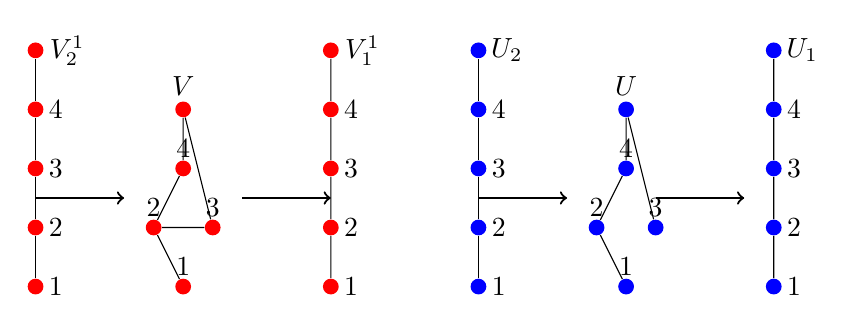
\begin{tikzpicture}[scale=0.75]
    % Left side: Search trees on K4
    \begin{scope}[every node/.style={circle,fill=red,inner sep=0pt, minimum size=0.2cm,text=black}]
        % First tree
        \node (1) at (0,0) [label=right:1] {};
        \node (2) at (0,1) [label=right:2] {};
        \node (3) at (0,2) [label=right:3] {};
        \node (4) at (0,3) [label=right:4] {};
        \node (V2) at (0,4) [label=right:$V_2^1$] {};
        \draw (1)--(2)--(3)--(4)--(V2);
        
        % Second tree
        \node (1b) at (2.5,0) [label=above:1] {};
        \node (2b) at (2,1) [label=above:2] {};
        \node (3b) at (3,1) [label=above:3] {};
        \node (4b) at (2.5,2) [label=above:4] {};
        \node (V) at (2.5,3) [label=above:$V$] {};
        \draw (1b)--(2b)--(4b)--(V)--(3b)--(2b);
        
        % Third tree
        \node (1c) at (5,0) [label=right:1] {};
        \node (2c) at (5,1) [label=right:2] {};
        \node (3c) at (5,2) [label=right:3] {};
        \node (4c) at (5,3) [label=right:4] {};
        \node (V1) at (5,4) [label=right:$V_1^1$] {};
        \draw (1c)--(2c)--(3c)--(4c)--(V1);
    \end{scope}
    
    % Arrows between trees
    \draw[->, thick] (0,1.5)--(1.5,1.5);
    \draw[->, thick] (3.5,1.5)--(5,1.5);
    
    % Right side: Images through π on SPK_{2,2}
    \begin{scope}[every node/.style={circle,fill=blue,inner sep=0pt, minimum size=0.2cm,text=black}, xshift=7.5cm]
        % First tree
        \node (1) at (0,0) [label=right:1] {};
        \node (2) at (0,1) [label=right:2] {};
        \node (3) at (0,2) [label=right:3] {};
        \node (4) at (0,3) [label=right:4] {};
        \node (U2) at (0,4) [label=right:$U_2$] {};
        \draw (1)--(2)--(3)--(4)--(U2);
        
        % Second tree
        \node (1b) at (2.5,0) [label=above:1] {};
        \node (2b) at (2,1) [label=above:2] {};
        \node (3b) at (3,1) [label=above:3] {};
        \node (4b) at (2.5,2) [label=above:4] {};
        \node (U) at (2.5,3) [label=above:$U$] {};
        \draw (1b)--(2b)--(4b)--(U)--(3b);
        
        % Third tree
        \node (1c) at (5,0) [label=right:1] {};
        \node (2c) at (5,1) [label=right:2] {};
        \node (3c) at (5,2) [label=right:3] {};
        \node (4c) at (5,3) [label=right:4] {};
        \node (U1) at (5,4) [label=right:$U_1$] {};
        \draw (1c)--(2c)--(3c)--(4c)--(U1);
    \end{scope}
    
    % Arrows between images
    \draw[->, thick] (7.5,1.5)--(9,1.5);
    \draw[->, thick] (10.5,1.5)--(12,1.5);
\end{tikzpicture}

\end{document}